\section{1985: New Computing Paradigm}
When micro-computers emerged around 1975, they were still used in the old way:
batch processing: Programs were activated one after another. A new paradigm
was pioneered in the Xerox Palo Alto Reserach Laboratory. The new facility of
high-resolution, bit-mapped displays called for a more flexible use of the screen.
So-called viewers, later windows, became available, and it was evident, that an
individual process should be attached to every viewers. The computer now allowed
the user to switch with every command from one viewer (process) to another. The
availability of a pointing device (mouse) facilitated this new paradigm: A mouse
click would replace the typing of an entire command.

Typing as such became less important. It was recognized that what was hitherto
typed, appeared somewhere in a viewer already. Thus, pointing at this text made
re-typing superfluous. One may claim that the viewer concept revolutionized
computer usage. It was a direct consequence of the new paradigm of object-oriented
programming: procedures (processes) can be attached to data structures. This
paradigm had already been introduced in the language Simula (1965), and later by
Smalltalk (1976), and the viewer concept is its most famous application. It was
perfected in Xerox' Cedar System and taken over in the Oberon system. Here the
notion of textual unit of program (the module) became clearly separated from the
unit of program execution (the procedure) contributing significantly to conceptual
clarity.
\begin{figure}[h!]
  \centering
  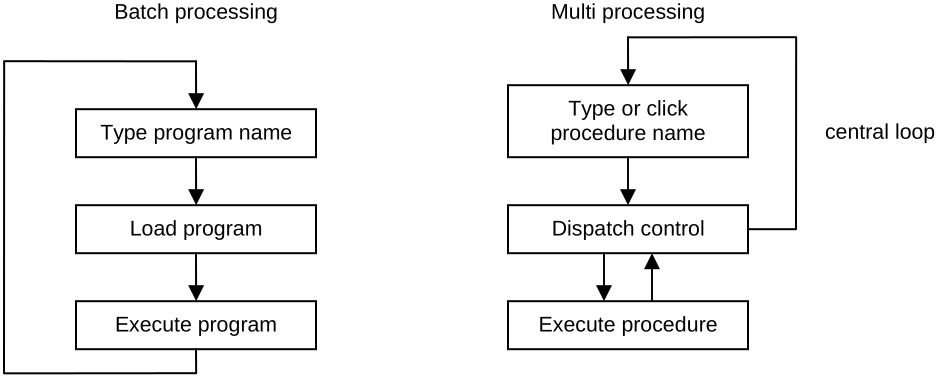
\includegraphics[width=\textwidth]{i/7}
\end{figure}

This entire progress was ultimately possible only due to the enormous increase in
memory size. When a procedure had been executed, it was not disposed from
memory, as was done in batch processing, but it was kept in memory to be quickly
accessible in a later call.
